\chapter{Rewriting systems}


Suppose a certain set of objects and a set of elementary transformations for these objects are given, and we are interested in the following problem.

\textit{Under what conditions do these transformations reduce each object to a single form?}

As we will see, this question is equivalent to an elegant statement about graphs (Lemma \ref{lem:diamond}).

For a precise formulation, we need to introduce rewriting systems.
They are understood in two senses: narrow and broad.
In the narrow sense, certain word transformations are considered.
These are the so-called \textit{string rewriting systems}, which will be defined in the next section.
In the broad sense, we talk about any objects and transformations; these are called \textit{abstract rewriting systems}.

\section{String rewriting systems}

Let us choose a finite set of symbols and call it an \index{alphabet}\emph{alphabet}.
Any finite strings (including the empty string) of symbols in the alphabet will be called a \index{word}\emph{word}.
If the alphabet has only two symbols $\{a,b\}$, then the words are 
$\emptyset$, $a$, $b$, $aa$, $ab$, $ba$, $bb$, $aaa$, and so on.

Suppose a list of pairs of words, $(s_1,t_1),\dots (s_n,t_n)$, is given;
we are allowed to change any occurrence of $s_i$ to $t_i$.
More precisely, a word $x=ls_ir$ can be exchanged for the word $y=lt_ir$;
here $l$ and $r$ are arbitrary words.
In this case we write $x\to y$.

For instance, we might be allowed to change $s_1=ba$ to $t_1=ab$ and $s_2=aba$ to $t_2=\emptyset$ anywhere in the word.
All possible words that can be reached from $bbaab$ are shown on the diagram.

{

\begin{wrapfigure}{o}{40 mm}
\vskip-0mm
\centering
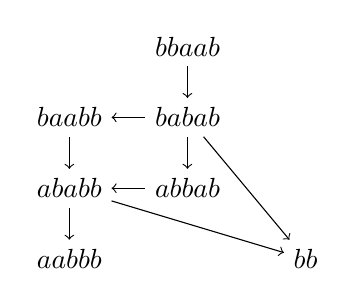
\begin{tikzpicture}[node distance=1.5cm, auto]
\node (bbaab) {$bbaab$};
\node (babab) [below of=bbaab, node distance=.9cm] {$babab$};
\node (abbab) [below of=babab, node distance=.9cm] {$abbab$};
\node (baabb) [left of=babab] {$baabb$};
\node (ababb) [left of=abbab] {$ababb$};
\node (aabbb) [below of=ababb, node distance=.9cm] {$aabbb$};
\node (b) [right of=aabbb] {};
\node (bb) [right of=b] {$bb$};
\draw[->] (bbaab) to (babab);
\draw[->] (babab) to (abbab);
\draw[->] (babab) to (baabb);
\draw[->] (babab) to (bb);
\draw[->] (ababb) to (bb);
\draw[->] (baabb) to (ababb);
\draw[->] (abbab) to (ababb);
\draw[->] (ababb) to (aabbb);
\end{tikzpicture}
\vskip-2mm
\end{wrapfigure}

We have just described the so-called \index{string rewriting system}\emph{string rewriting systems}.
To describe the given example, we will use the notation
\[\langle\, a,b \mid ba\to ab,\, aba\to\emptyset\,\rangle.\]
So, after $\langle$, we list the symbols of the alphabet, and after $\mid$, we list all allowed replacements, closing it with $\rangle$.

}

\section{Abstract rewriting systems}

An \index{abstract rewriting system}\emph{abstract rewriting system} is a \index{digraph}\emph{digraph};
that is, a pseudograph (typically infinite) on each edge of which one of two directions is chosen.
The vertices of the digraph are often referred to as \index{object}\emph{objects}, and directed edges as \index{transformation}\emph{transformations}.
For two objects $x$ and $y$, we write $x \to y$ if there is a directed edge that starts at vertex $x$ and ends at vertex $y$; it defines a relation on the set of objects.

We will be interested in the relation $\to$ on the set of vertices.
Of course, if we know the digraph, then we know the relation $\to$.

A string rewriting system can be interpreted as an abstract rewriting system with the set of vertices formed by
all words in the alphabet.

Let us introduce two new binary relations on the set of vertices of the digraph that will be denoted by $\rightsquigarrow$ and $\sim$.

The first relation $x\rightsquigarrow y$ means that following the arrows in the digraph,
one can get from $x$ to $y$; it includes the case $x=y$.
More precisely, there is a sequence of objects $x=x_0\to x_1\to\dots\to x_n=y$ for some integer $n\ge 0$.

The expression $x \sim y$ says that one can walk along edges in the digraph from $x$ to $y$;
it is allowed to go in both directions of the edges.
In other words, $x \sim y$ means that $x$ and $y$ lie in the same connected component of the undirected pseudograph.

\section{Terminating systems}

A system is called \index{terminating system}\emph{terminating} if there are no infinite sequences $x_0 \to x_1 \to \dots $
In other words, one cannot travel around the digraph indefinitely, following the directions of the arrows.

An object $w$ (a vertex) is said to be \index{irreducible object}\emph{irreducible} if there is no object $x$ such that $w \to x$.
In other words, there is no way out of $w$.

It is clear that in a terminating rewriting system, starting at vertex $x$ and traveling along the arrows, we will arrive at some irreducible vertex, say~$w$.
In the latter case, we will say that $w$ is a \index{normal form}\emph{normal form} of $x$.

Any object in the terminating system has at least one normal form, and there can be many of them.
If $x$ has a {}\emph{unique normal form}, then it will be denoted by \index{$[x]$ (normal form)}$[x]$.



\begin{thm}{Exercise}\label{ex:examples}
Give an example of 
\begin{enumerate}[(a)]
\item a finite nonterminating system.
\item a terminating system such that a vertex $v_0$ has an arbitrary long sequence $v_0 \to v_1 \to \dots \to v_n$.
\item an infinite nonterminating  system such that any object has a unique normal form.
\end{enumerate}

\end{thm}

\section{Confluent systems}

\begin{wrapfigure}{r}{20 mm}
\vskip-0mm
\centering
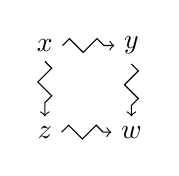
\begin{tikzpicture}[node distance=1.1cm, auto]
\node (x) {$x$};
\node (zz) [below of=x] {$z$};
\node (yy) [right of=x] {$y$};
\node (v) [below of=yy] {$w$};
\draw[->,decorate,decoration=zigzag] (x) to (zz);
\draw[->,decorate,decoration=zigzag] (x) to (yy);
\draw[->,decorate,decoration=zigzag] (yy) to (v);
\draw[->,decorate,decoration=zigzag] (zz) to (v);
\end{tikzpicture}
\vskip-0mm
\end{wrapfigure}

A system is called \index{confluent system}\emph{confluent} if the conditions $x\rightsquigarrow  y$ and $x\rightsquigarrow  z$
for any three objects $x$, $y$, $z$ imply that
there is an object $w$ such that $y\rightsquigarrow  w$ and $z\rightsquigarrow  w$.
Informally, it means that if two people start at $x$ and follow the arrows for some time,
then, going further along the arrows, they can always converge at some vertex $w$.


\begin{thm}{Lemma}\label{lem:x->y}
Suppose two objects $x$ and $y$ in a confluent system have normal forms 
$v$ and $w$, respectively.
If $x\rightsquigarrow y$, then $v=w$.
\end{thm}

\parit{Proof.}
Since $x\rightsquigarrow y$ and $x\rightsquigarrow v$, we get $v\rightsquigarrow v'$ and $y\rightsquigarrow v'$ for some object $v'$.
Since $v$ is irreducible, we get $v=v'$;
that is $y\rightsquigarrow v$.

Since $y\rightsquigarrow v$ and $y\rightsquigarrow w$, we get $v\rightsquigarrow w'$ and $w\rightsquigarrow w'$ for some object $w'$.
Since $v$ and $w$ are irreducible, we get $v=w'=w$.
\qeds

A terminating confluent system is called \index{convergent}\emph{convergent}.

\begin{thm}{Theorem}
In a convergent system, any object has a unique normal form.
Moreover, for any two objects $x$ and $y$ in the system we have
\[x\sim y\qquad\Longleftrightarrow\qquad [x]=[y].\]

\end{thm}

\parit{Proof.}
Since the system is terminating, any object $x$ has a normal form.

Let $y$ and $z$ be normal forms of $x$;
in particular $x\rightsquigarrow y$ and $x\rightsquigarrow z$.
Since the system is confluent, $y\rightsquigarrow w$ and $z\rightsquigarrow w$ for some object $w$.
However, since both objects $x$ and $y$ are irreducible, we have $y= w$ and $z= w$;
that is, any object $x$ has a unique normal form, which proves the main statement.

Suppose $w=[x]=[y]$.
Then $x\rightsquigarrow w$ and $y\rightsquigarrow w$.
Therefore, $x\sim y$;
we proved the if part of the second statement.

Now suppose $x\sim y$;
so there is a sequence $x=x_0,x_1,\dots,x_n=y$ such that $x_i\to x_{i+1}$ or $x_{i+1}\to x_i$ for each $i$.
By \ref{lem:x->y},
\[[x]=[x_0]=[x_1]=\dots=[x_n]=[y].\]
Hence the only-if part follows.
\qeds

\section{Proving termination}

So, how do we prove that a system is terminating?
Typically, we construct a relation ``$\succ$'' on the set of vertices such that 
$x \to y$ implies $x\succ y$.
If any decreasing sequence with respect to $\succ$ is terminating,
then our original system is terminating as well. 

More precisely, ``$\succ$'' is a strict partial order;
that is, ``$\succ$'' is a relation that satisfies the following conditions for all objects $x$, $y$, and $z$:
\begin{itemize}
\item $x\nsucc x$.
\item If $x\succ y$, then  $y\nsucc x$.
\item If $x\succ y$ and $y\succ z$ then  $x\succ z$.
\end{itemize}
If there is no infinite sequence $x_0\succ x_1\succ\dots$,
and $x\to y$ implies $x\succ y$, then our system is terminating.

\begin{thm}{Exercise}\label{ex:x+1}
Let $A$ be an abstract rewriting system
with a set of objects formed by positive integers 
and the transformations $x\to \tfrac x2$ if $x$ is even and $x\to x+1$ if $x>1$ is odd.
Show that $A$ is terminating.
\end{thm}

For string rewriting systems, the words can be ordered first by length, and if the lengths are equal, lexicographically.
This is the so-called \index{shortlex order}\emph{shortlex order}.
Note that for this order, there is no infinite decreasing sequence.
In this case, to ensure that the system is terminating, it is sufficient that when moving from one word to another along the arrow, either the length of the word decreases, or it does not change, but the word decreases relative to the order of words in the dictionary.

\begin{thm}{Exercise}\label{ex:balls}
Show that the following process always terminates.
There is a box with a finite number of black and white balls.
Each step consists of removing an arbitrary ball from the box.
If it happens to be a black ball, one also adds an arbitrary (but finite) number of white balls to the box.
\end{thm}

\begin{thm}{Exercise}\label{ex:ab>ba,aba>}
Show that the following string rewriting system 
\[\langle\, a,b \mid ba\to ab,\, aba\to\emptyset\,\rangle\]
is terminating.
\end{thm}


\section{Proving confluence}

Checking confluence is a more difficult problem.
One needs to keep track of all pairs of paths leaving the same vertex.
It turns out that this is not necessary.

\begin{wrapfigure}{r}{20 mm}
\vskip-0mm
\centering
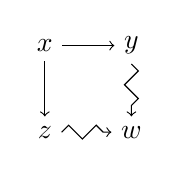
\begin{tikzpicture}[node distance=1.1cm, auto]
\node (x) {$x$};
\node (zz) [below of=x] {$z$};
\node (yy) [right of=x] {$y$};
\node (v) [below of=yy] {$w$};
\draw[->] (x) to (zz);
\draw[->] (x) to (yy);
\draw[->,decorate,decoration=zigzag] (yy) to (v);
\draw[->,decorate,decoration=zigzag] (zz) to (v);
\end{tikzpicture}
\vskip-0mm
\end{wrapfigure}

An abstract rewriting system is called \index{locally confluent}\emph{locally confluent} if for any objects $x$, $y$, $z$, from the conditions $x \to y$, $x\to z$, follows the existence of an object $w$ such that $y\rightsquigarrow  w$, $z\rightsquigarrow  w$.
This means that if two people started from the same vertex and each walked along one directed edge, then they can converge somewhere, following the arrows.

It is clear that every confluent system is locally confluent.

\begin{thm}{Exercise}\label{ex:not-confluent}
Construct a system that is locally confluent but not confluent.
\end{thm}


\begin{thm}{Diamond lemma}\label{lem:diamond}
A terminating rewriting system is confluent if and only if it is locally confluent.
\end{thm}
 

Let us describe an induction-type argument that will be used in the proof.

Suppose we want to prove a statement $P(x)$ for every object $x$ of the terminating system.
Then it is sufficient to prove the induction step:
\textit{$P(x)$ holds under the assumption that $P(y)$ holds for all downstream objects $y$}.
In other words, we need to show that \textit{if $P(y)$ holds for any object $y\ne x$ such that $x\rightsquigarrow y$, then $P(x)$ holds as well}.

Let us explain why it works.
Suppose we proved the induction step for some statement $P$ in a terminating system, but $P(x_0)$ does not hold for an object $x_0$.
Then we may choose another object $x_1\ne x_0$ such that $P(x_1)$ does not hold and $x_0\rightsquigarrow x_1$.
Continuing this way, we get an infinite descending sequence $x_0\rightsquigarrow x_1\rightsquigarrow x_2\dots$ of so that $x_0\ne x_1$, $x_1\ne x_2$, and so on.
The latter contradicts that our system is terminating.

Note that applying the step of induction to the empty set of objects,
we get that $P(x)$ holds for any irreducible object, and we can continue further.
It explains why this version of induction requires no base.

\parit{Proof.}
The only-if part is trivial;
let us prove the if part.

Given an object $x$, we need to show that if $x\rightsquigarrow y$ and $x\rightsquigarrow  z$, then there is $w$ such that $y\rightsquigarrow w$ and $z\rightsquigarrow  w$.
Denote the latter statement by $P(x)$.

If $x=y$ or $x=z$, then there is nothing to prove.
Therefore, we can assume that $x\ne y$ and $x\ne z$.
Consider the first edges $x\to y'$ and $x \to z'$ of the paths defining $x\rightsquigarrow y$ and $x\rightsquigarrow  z$; 
so we have $x\to y'$, $y' \rightsquigarrow  y$, $x \to z'$, and $z' \rightsquigarrow  z$.

\begin{wrapfigure}[9]{r}{40 mm}
\vskip-6mm
\centering
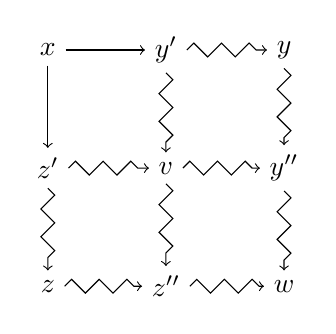
\begin{tikzpicture}[node distance=1.5cm, auto]
\node (x) {$x$};
\node (zz) [below of=x] {$z'$};
\node (z) [below of=zz] {$z$};
\node (zzz) [right of=z] {$z''$};
\node (yy) [right of=x] {$y'$};
\node (y) [right of=yy] {$y$};
\node (yyy) [below of=y] {$y''$};
\node (v) [below of=yy] {$v$};
\node (w) [below of=yyy] {$w$};
\draw[->] (x) to (zz);
\draw[->] (x) to (yy);
\draw[->,decorate,decoration=zigzag] (yy) to (y);
\draw[->,decorate,decoration=zigzag] (yy) to (v);
\draw[->,decorate,decoration=zigzag] (zz) to (v);
\draw[->,decorate,decoration=zigzag] (zz) to (z);
\draw[->,decorate,decoration=zigzag] (z) to (zzz);
\draw[->,decorate,decoration=zigzag] (v) to (zzz);
\draw[->,decorate,decoration=zigzag] (v) to (yyy);
\draw[->,decorate,decoration=zigzag] (y) to (yyy);
\draw[->,decorate,decoration=zigzag] (zzz) to (w);
\draw[->,decorate,decoration=zigzag] (yyy) to (w);
\end{tikzpicture}
\vskip-0mm
\end{wrapfigure}

Applying the local confluence condition to a pair of edges $x \to y'$, $x \to z'$, we find a vertex $v$ such that $y' \rightsquigarrow  v$ and $z' \rightsquigarrow  v$.

Next, the vertices $y'$ and $z'$ are descending with respect to $x$, and the same applies to vertex $v$. Therefore, by the induction hypothesis, the statements $P(y')$, $P(z')$, and $P(v)$ hold true.

Since $y' \rightsquigarrow  y$ and $y' \rightsquigarrow  v$ we can get $y''$ such that $y\rightsquigarrow  y''$ and $v\rightsquigarrow y''$.
Likewise, we get $z''$ such that $z\rightsquigarrow  z''$ and $v\rightsquigarrow  z''$.

Finally, we use $P(v)$.
Since $v\rightsquigarrow  y''$ and $v \rightsquigarrow z''$, we can find $w$ such that $y'' \rightsquigarrow  w$ and $z'' \rightsquigarrow  w$.

Finally, $y \rightsquigarrow y'' \rightsquigarrow  w$ implies $y \rightsquigarrow  w$.
Likewise, we get $z \rightsquigarrow  w$.
\qeds

\section{Applications}

Suppose $x$ is a word in a string rewriting system
from which two arrows emanate $x\to y$ and $x\to z$.
So, $y$ and $z$ are obtained from $x$ by two elementary transformations, replacing some of its occurrences $s_i$ and $s_j$ with $t_i$ and $t_j$, respectively.
If occurrences do not overlap, then we can apply these two transformations in any order and get the same result, say $w$.
In this case, local confluence holds.

If the occurrences overlap, then two cases are possible:
they can either be contained in one another (a rarer case) or overlap by some non-empty word.
Without loss of generality, we can pass to the part of our word that is the union of occurrences $s_i$ and $s_j$.
The following two cases are subject to verification.

\parit{Case A.} Suppose $s_{i}$ and $s_j$ overlap by non-empty word $q$;
we may assume that  $s_{i}=lq$ and  $s_{j}=qr$, for some words $l$ and $r$.
That is, we have a word $lqr$, from which we can go along the edge to both the word $t_{i}r$ and the word $lt_{j}$.
By making transformations in these words, we want to reduce them to one word; that is, we need to find a word $w$ such that $t_{i}r\rightsquigarrow  w$ and $lt_{j}\rightsquigarrow w$.

\parit{Case B.} Suppose  $s_{j}$ is contained in $s_{i}$;
in other words $s_i=ls_{j}r$ for some words $l$ and $r$.
In this case, from the vertex $s_{i}$ we can move along the edge to both $t_{i}$ and $lt_{j}r$.
The goal is to find a word $w$ such that $t_{i}\rightsquigarrow w$, $lt_{j}r\rightsquigarrow w$.


\begin{thm}{Example}\label{em:baaba>a}
\[\langle a,b \mid baaba\to a\rangle.\]
\end{thm}

Applying the shortlex order, we find that the system is terminating.

To check confluence, we need to examine cases A and B.
There is only one word here, but it overlaps with itself in $ba$.
By gluing together two such words that overlap in $ba$, we come to checking the word $baabaaba$.
Applying the transformation at the left and right ends, we get two irreducible words
$aaba$ and $baaa$.
It follows that the system is not confluent and, therefore, not convergent.

\medskip

In this example, the words $aaba$ and $baaa$ are equivalent to the original word $baabaaba$.
Therefore, if we add $baaa\to aaba$ to the existing rules, then the word equivalence relation will remain unchanged.
It leads to the following example.

\begin{thm}{Example}\label{em:baaba>a,baaa>aaba}
\[\langle a, b \mid baaba\to a, baaa\to aaba\rangle.\]
\end{thm}

Again, applying the shortlex order, we find that the system is terminating.

Now we need to go thru all the options for overlapping words.
There are only two such options.
One of them is old and does not need to be checked.
Now the words $aaba$ and $baaa$ from the previous example are automatically converted to $aaba$ in the new system.
But we have a new relationship, and therefore a new overlap has arisen: $baaba$ overlaps with $baaa$ by $ba$. (Here you must always be careful, since a new word can give several new overlaps;
two words can overlap not in one, but in many ways --- all this must be checked.)

Gluing the overlapping words together leads to $baabaaa$
and we can get $(baaba)aa\to aaa$
and $baa(baaa)\to baaaaba$.
Since $(baaa)aba \z\to  aa(baaba) \to aaa$, we get that the system is confluent,
and therefore convergent.

\begin{thm}{Exercise}\label{ex:convergent}
Check if the following systems are terminating and conluent.

\begin{enumerate}[(a)]
 \item\label{ex:convergent:a} \[\langle a, b \mid baaba\to a, aaba \to  baaa\rangle;\]
 \item\label{ex:convergent:b} \[\langle a,b,c \mid ba\to ab, ca\to ac, cb\to bc \rangle;\]
 \item\label{ex:convergent:c} \[\left\langle
\begin{matrix}
x,&y,&z,
\\
X,&Y,&Z
\end{matrix}
\,
\middle| 
\,
\begin{matrix}
xX\to \emptyset,& yY\to \emptyset,& zZ\to \emptyset,
\\
Xx\to \emptyset,& Yy\to \emptyset,& Zz\to \emptyset
\end{matrix}
\,
\right\rangle.\]
\end{enumerate}

\end{thm}

\section{Comments}

This chapter is inspired by a blog post by Victor Guba \cite{guba}.
Several examples and exercises are taken from the book by Franz Baader and Tobias Nipkow \cite{baader-nipkow},
which is very good for further study.

The diamond lemma (\ref{lem:diamond}) is also known as \index{Newman's lemma}\emph{Newman's lemma};
it was proved by Max Newman \cite[Theorem 3]{newman}.

The replenishment of the system in \ref{em:baaba>a} to the system in \ref{em:baaba>a,baaa>aaba} is called  the \index{Knuth--Bendix procedure}\emph{Knuth--Bendix procedure}.
In our example, we get a convergent system in one step.
In general, to obtain a convergent system, one may need to apply the procedure several times, but this process may also run forever.




